% EE604 course project. Camera-ready CVPR format: authors are visible,
% and the review ruler is off.

\documentclass[10pt,twocolumn,letterpaper]{article}

\usepackage[pagenumbers]{cvpr}
\usepackage{amsmath}
\usepackage{amssymb}
\usepackage{graphicx}
\usepackage{booktabs}
\usepackage{tikz}
\usetikzlibrary{positioning,arrows.meta}
\usepackage{listings}

\lstset{
  language=Python,
  basicstyle=\ttfamily\scriptsize,
  breaklines=true,
  columns=fullflexible,
  keepspaces=true,
  showstringspaces=false,
  frame=single,
  numbers=left,
  numberstyle=\tiny\color{black},
  tabsize=4,
  captionpos=b
}

\graphicspath{{../experiments/results/}}


\definecolor{cvprblue}{rgb}{0.21,0.49,0.74}
\usepackage[pagebackref,breaklinks,colorlinks,allcolors=cvprblue]{hyperref}

\def\confName{CVPR}
\def\confYear{2026}

\title{Orientation-Aware Seam Carving for Image Retargeting}

\author{230991\\
EE604, Department of Electrical Engineering\\
Indian Institute of Technology Kanpur
}

\begin{document}
\maketitle

\begin{abstract}
Image retargeting changes the height and width of a photograph so that it fits a new layout while the objects a viewer would notice, and the long straight structures in the scene, stay intact.
Uniform scaling compresses the whole frame, and a center crop throws away everything outside a window.
This project instead deletes or duplicates low-cost seams.
The seam cost is the forward energy of Rubinstein, Shamir, and Avidan, which charges the new edges a deletion would create, plus two maps: spectral-residual saliency, and a line map whose weight depends on the direction of the seam. A pretrained salient-object model is an optional comparison and is not the default cost.
Vertical seams are discouraged from cutting vertical structures, and horizontal seams from cutting horizontal ones.
On eight images from the RetargetMe benchmark, the combined cost is compared with scaling, center-cropping, classic backward-energy seams, and ablations that turn saliency or lines off.
Against forward energy alone, on eight images at a 25\% width reduction, the saliency weight lowers the mean deleted spectral-residual fraction from 0.089 to 0.068, and the line weight lowers crossings of the same line map from 1.14 to 0.31 per 100 seam pixels.
On the seeded 30 images that saliency reduction holds: the full model is 0.093 (0.031) against 0.118 (0.037) for classic seams, lower on all 30 (two-sided sign test $p = 1.86 \times 10^{-9}$).
The full model matches the saliency-only score and sits a little above the lines-only score, at 0.37 rather than 0.31.
The saliency and Hough line scores reuse the maps inside the cost, so they show that the weights move the seams.
On those eight, an LSD map that is not in the cost shrinks the line-score gap from about 72\% to about 13\%, and the full model is lower on only four images.
That drop does not hold on a seeded sample of 30 RetargetMe images.
The draw, seed 604, did not include Johanneskirche or \texttt{obama}.
At 75\% width the full model's LSD score is 1.26 (1.10) against 1.08 (0.93) for classic seams, lower on 12 images, higher on 17, and tied on one (two-sided sign test $p = 0.46$).
Forward energy alone is 1.35 (1.37), and adding the line weight leaves 1.16 (0.94), lower on 16, higher on 13, and tied on one ($p = 0.71$).
These scores are not a measure of whether the picture looks better.
At 75\% width the two seam results look similar.
A center crop already removes off-center content, and a 50\% cut of a curved sculpture pinches it under both seam methods.
A hybrid schedule uses the same cost but stops the seams at 75\% of the original side and scales the rest.
The 50\% result is then the 75\% seam image scaled down.
It does not add the further pinching that comes from carving all the way to half width, and it still does not match uniform scaling, which never cuts the sculpture.
\end{abstract}

\section{Introduction}
Photographs are displayed at aspect ratios their cameras did not use: a phone story, a banner, a slide, a print.
The operation that produces the new size is image retargeting.
Its input is one color image, a target height, and a target width.
Its output is an image of that exact size.
The constraint in this project is that the computation stays in the spatial domain.
There is no trained retargeting network. A pretrained salient-object model is an optional comparison and is not the default cost.
The implementation uses NumPy 2.5.4, OpenCV 5.0.0, and, only for that comparison, rembg 2.0.86 with onnxruntime 1.29.0 and the u2netp checkpoint (4574861 bytes). The dynamic program runs on images whose long side is at most 640 pixels so that a demo can recompute a result on request.

Two standard operators ignore content.
Scaling moves every pixel by the same factor, so a face becomes thinner when the frame becomes narrower.
Cropping keeps a window and discards the rest, so an off-center subject can disappear even though the remaining pixels look sharp.
Seam carving~\cite{avidan2007seam} takes a third route.
A vertical seam is an 8-connected path of one pixel per row.
Deleting the cheapest such paths changes the width without a global resample.
The original cost is a backward energy: the gradient magnitude of the pixels that are removed.
That cost does not look at the tear those pixels leave behind, and a smooth subject can be cheaper to cut than a textured background.

Forward energy~\cite{rubinstein2008improved} fixes the tear by scoring the edges that appear after the deletion.
It still has no notion of a person or of a window mullion.
The default saliency term raises the cost of pixels that the spectral residual marks. Those pixels are often edges, not a detected person. The optional learned map is a pretrained salient-object model.
A line map raises the cost of long straight segments.
Both ideas exist in the literature as separate add-ons.
The variant defended here puts them in one recurrence, and it does not treat every line the same way.
A vertical seam is allowed to cross a horizon, because every vertical seam must, and it is penalized for crossing a column or a mullion.
A horizontal seam swaps that preference.
Section~\ref{sec:method} defines the cost.
Section~\ref{sec:exp} compares it with scaling, cropping, and classic seams, and turns each extra term off in an ablation.

\section{Related work}
Avidan and Shamir~\cite{avidan2007seam} select seams by dynamic programming on an energy map, remove them to shrink, and duplicate them to enlarge.
The energy they use is a function of the image gradient.
Rubinstein, Shamir, and Avidan~\cite{rubinstein2008improved} replace that energy with a forward cost that depends on which neighbor the seam arrives from, because the pixels that become adjacent are not known from the gradient alone.
The same authors later choose among scaling, cropping, and seam carving with a multi-operator search~\cite{rubinstein2009multi}.
We do not search over operators.
Scaling and cropping are baselines, and the seam operator is fixed.

Hou and Zhang~\cite{hou2007saliency} define a saliency map from the spectral residual of the Fourier amplitude.
The residual is the log amplitude minus a local average of the log amplitude, combined with the original phase.
The map needs no training images.
RetargetMe~\cite{rubinstein2010comparative} is the public benchmark used below.
It compares several retargeting operators with a user study.
We report automatic scores and side-by-side figures on a subset of its source images, and we do not repeat that user study.

\section{Method}
\label{sec:method}

Figure~\ref{fig:overview} is the pipeline.
Luminance is computed once per seam from the current color image.
Saliency and the two line maps are computed once on the image at the start of a shrinking or enlarging stage.
When a seam is deleted, the same pixel indices are deleted from those maps.
Forward energy is not stored.
It is recomputed from the current luminance inside the dynamic program, because it depends on the neighbors that still exist.

\begin{figure}[t]
\centering
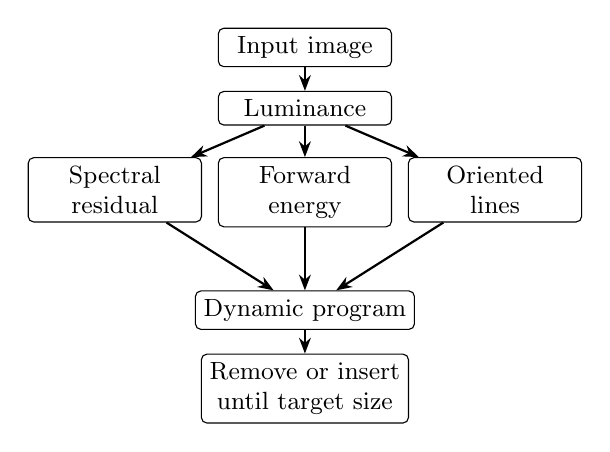
\begin{tikzpicture}[
  font=\small,
  box/.style={draw, rounded corners=2pt, align=center, inner sep=3pt, minimum width=22mm},
  arr/.style={-{Stealth[length=2mm]}, thick}
]
\node[box] (in) {Input image};
\node[box, below=3mm of in] (y) {Luminance};
\node[box, below left=4mm and 2mm of y] (sal) {Spectral\\residual};
\node[box, below=4mm of y] (fwd) {Forward\\energy};
\node[box, below right=4mm and 2mm of y] (lin) {Oriented\\lines};
\node[box, below=8mm of fwd] (dp) {Dynamic program};
\node[box, below=3mm of dp] (out) {Remove or insert\\until target size};
\draw[arr] (in) -- (y);
\draw[arr] (y) -- (sal);
\draw[arr] (y) -- (fwd);
\draw[arr] (y) -- (lin);
\draw[arr] (sal) -- (dp);
\draw[arr] (fwd) -- (dp);
\draw[arr] (lin) -- (dp);
\draw[arr] (dp) -- (out);
\end{tikzpicture}
\caption{Overview. Forward energy is evaluated on the current luminance. Saliency and the line maps travel with the pixels as seams are removed.}
\label{fig:overview}
\end{figure}

\subsection{Saliency and line protection}
Luminance is the Rec.\ 601 combination $Y = 0.299R + 0.587G + 0.114B$, scaled to $[0,1]$.
Spectral residual saliency follows Hou and Zhang.
The log amplitude of the Fourier transform is subtracted from its $3\times 3$ local average, the original phase is kept, and the inverse transform is squared, blurred with a Gaussian of standard deviation 2.5, and normalized to $[0,1]$.

Line segments come from a blurred Canny edge map and the probabilistic Hough transform.
The blur (a $5\times 5$ Gaussian with $\sigma = 1.2$) and the Canny thresholds (80 and 160) are there so that brick texture does not fill the mask.
A segment is kept only when it is at least 30 pixels long and at least 12\% of the short side.
At most 40 of the longest segments are drawn, with thickness 2.
Let $\theta$ be the segment angle from the $x$-axis.
For a vertical seam, which changes the width, the segment is drawn with weight $|\sin\theta|$.
A vertical mullion then has weight 1, and a horizontal horizon has weight 0.
For a horizontal seam the weight is $|\cos\theta|$.
Overlapping draws keep the per-pixel maximum.
The horizon still has to be crossed by every vertical seam.
The weight stops that forced crossing from also penalizing columns and poles.

\subsection{Dynamic program}
Index rows by $i$ and columns by $j$, and write $I$ for the current luminance.
The forward costs of arriving at $(i,j)$ from the three pixels in the row above are
\begin{align}
C_U(i,j) &= \lvert I(i,j{+}1) - I(i,j{-}1) \rvert, \label{eq:cu}\\
C_L(i,j) &= C_U(i,j) + \lvert I(i{-}1,j) - I(i,j{-}1) \rvert, \label{eq:cl}\\
C_R(i,j) &= C_U(i,j) + \lvert I(i{-}1,j) - I(i,j{+}1) \rvert. \label{eq:cr}
\end{align}
$C_U$ is the new edge between the left and right neighbors that the deletion joins.
$C_L$ and $C_R$ add the edge against the pixel the seam just left when the step is diagonal.
Out-of-range neighbors are clamped to the border pixel.
A step that would leave the image is given infinite cost.
The direction-independent term is the saliency $S$ and the line map $L_d$ for the seam direction $d$,
\begin{equation}
E(i,j) = w_s S(i,j) + w_l L_d(i,j).
\label{eq:extra}
\end{equation}
The cumulative cost and the chosen step are
\begin{equation}
\begin{aligned}
M(i,j) = E(i,j) + \min\big\{
&M(i{-}1,j{-}1)+C_L,\\
&M(i{-}1,j)+C_U,\\
&M(i{-}1,j{+}1)+C_R
\big\}.
\end{aligned}
\label{eq:dp}
\end{equation}
The first row is $M(0,j) = E(0,j)$.
Backtracking from the minimum of the last row yields one column index per row.
Consecutive indices differ by at most one, so the seam is 8-connected.
The weights used for every reported number are $w_s = 0.5$ and $w_l = 0.8$.
They were chosen by looking at Johanneskirche and \texttt{obama}, which are two of the eight evaluation images, and then frozen.
There is no weight sweep.
The demo sliders can still override them.
Section~\ref{sec:exp} also reports the means with those two images removed, as a sensitivity check rather than a held-out tuning.

Classic seam carving uses the same backtracking with a different recurrence.
Its pixel cost is the sum of absolute Sobel responses, and it has no forward term and no saliency or line term.
Horizontal seams are vertical seams on the transposed image, with the matching line map transposed as well.
While both the height and the width are still above the target, the algorithm computes one seam in each direction and deletes the cheaper one.
Enlargement records the seams that would be removed, maps their indices back onto the image before insertion, and writes an averaged copy of each seam pixel next to its right neighbor.
One recording pass inserts at most $W-2$ seams, which can almost double the width.
The $1.5\times$ enlargement in the experiments fits in that single pass.
A second pass runs only when the target is wider than $2W-2$.

\subsection{Hybrid schedule}
The full model above carves until the image is the requested size.
On a deep shrink that is where curved, busy scenes tear: each new seam is still the cheapest path, and after the easy background is gone the path goes through the object.
The hybrid operator keeps Equation~\eqref{eq:dp} and the same weights, and changes only when scaling takes over.
If a target side is at least 75\% of the original, hybrid is the full model and does not scale.
If the target is smaller, seams stop at $\mathrm{round}(0.75 \times \text{original})$ and \texttt{cv2.resize} finishes that side.
A request for 50\% width therefore deletes columns by seams until the width is 75\% of the original, then resizes that image to 50\%.
Enlargement is unchanged.
This is a fixed schedule, not a search over operators~\cite{rubinstein2009multi}.
An edge-density term was tried informally as a way to protect curves and then left out of the cost.
It was not measured, and there is no figure for it.
A vertical seam crosses a curved outline in a few rows and then travels through the smooth interior, so raising the outline can move the seam into that interior.
Figure~\ref{fig:maps} shows the saliency map, the line map, and the next seam on Johanneskirche.
The Hough line map in the cost is unchanged.
OpenCV's line-segment detector is not substituted into that cost.
Section~\ref{sec:exp} still scores the Hough map, and it also counts the same seams on a separate LSD map that does not choose them.

\begin{figure*}[t]
\centering
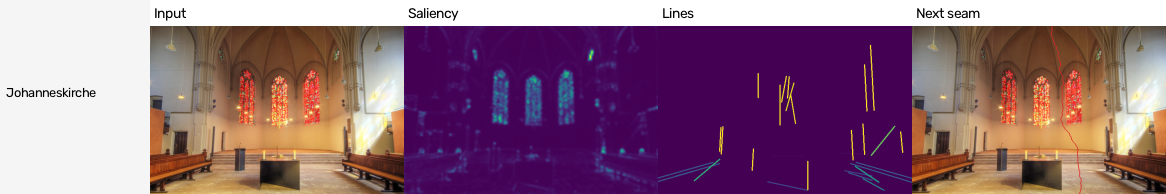
\includegraphics[width=\textwidth]{fig_maps.png}
\caption{Maps on Johanneskirche, the line example. Left to right: the working image, spectral-residual saliency, the line map used by vertical seams (bright yellow marks near-vertical segments), and the next seam chosen by the full model.}
\label{fig:maps}
\end{figure*}

\section{Experiments}
\label{sec:exp}

\subsection{Data and implementation}
The images are eight source photographs from RetargetMe~\cite{rubinstein2010comparative}: \texttt{obama} and \texttt{child} (people), \texttt{brick\_house} and \texttt{Johanneskirche} (buildings), \texttt{eagle} and \texttt{butterfly} (compact objects), \texttt{waterfall} (a landscape), and \texttt{Sanfrancisco} (a busy outdoor scene).
The download script keeps these eight files from the public source-image archive and does not redistribute the other 72.
Before any operator runs, the long side is limited to 640 pixels with area interpolation.
The code is Python 3 with NumPy and OpenCV.
No GPU is used.
The row update of the dynamic program is vectorized across the width.

Five operators are compared.
\textbf{Scale} is \texttt{cv2.resize} to the exact target, with area interpolation when both sides shrink.
\textbf{Crop} cuts the centered window of the target aspect ratio and then resizes it to the exact target.
\textbf{Classic} is backward-energy seam carving.
\textbf{Ours} is Equation~\eqref{eq:dp} with $w_s = 0.5$ and $w_l = 0.8$.
\textbf{Hybrid} is that same cost, with seams stopped at 75\% of the original side and a uniform scale after that.
At a 75\% target the two are the same operator.
Hybrid is reported on the 50\% width cut.
The ablation uses the same recurrence with $(w_s, w_l)$ set to $(0,0)$ (forward energy alone), $(0.5, 0)$ (saliency only), and $(0, 0.8)$ (lines only).

The width is reduced to 75\% and to 50\% of the working width, with the height held fixed.
The 75\% setting is a 25\% reduction and is the one used for the ablation and the runtime.
\texttt{waterfall} is also reduced to 75\% height, and \texttt{butterfly} is enlarged to 150\% width.
Every reported output was checked to have the requested height and width.

Three seam scores are reported.
The saliency fraction is the sum of the spectral-residual map on pixels that are actually deleted, divided by the sum of that map.
Insertion does not delete pixels, so the fraction is not used for the enlargement.
The Hough line score is the number of seam pixels that land on a positive value of the Hough map, per 100 seam pixels.
The LSD line score is the same count on an LSD map.
The saliency fraction and the Hough score use maps that the full model puts in its cost.
The LSD map does not.
Classic seams are scored with those maps even though their recurrence does not use them.
A lower number therefore shows that the weight changed which pixels were deleted.
It does not, by itself, show that a viewer would prefer the result, and it does not measure tears in regions the maps do not mark.
Scale and crop do not choose seams, so they have no entry on these three scores.
Runtime is one wall-clock measurement of the whole call.
Before the 30-image sample, the original eight were carved again at 75\% width.
The saliency fraction and the Hough score matched \texttt{metrics.csv} on every seam method, including \texttt{brick\_house} classic at 0.153154 and 3.2319.
That sample is 30 source images drawn with seed 604.
Three of those 30 are also in the original eight: \texttt{child}, \texttt{Sanfrancisco}, and \texttt{waterfall}.
LSD is counted in the same pass that chooses the seams.
The run writes a CSV only.
Contact sheets stay the original eight.

\subsection{Results}
Table~\ref{tab:width75} gives the mean and sample standard deviation at 75\% width.
Those standard deviations, Table~\ref{tab:perimage}, and the six-image check later in this section are the printout of \texttt{experiments/report\_numbers.py} on the saved \texttt{metrics.csv}.
They are the worked example.
Table~\ref{tab:n30} and the sign tests below it are the printout of \texttt{experiments/run\_n30.py}, saved as \texttt{n30\_summary.txt}.
Table~\ref{tab:width50} is the 50\% width cut.
Table~\ref{tab:perimage} is the per-image breakdown at 75\% width.
Figure~\ref{fig:compare75} shows four of the eight images at 75\% width: the church (lines), the portrait (saliency), the street sculpture (a busy scene), and the waterfall.
Figure~\ref{fig:compare50} repeats that set at 50\% width.
Figure~\ref{fig:ablation} isolates the terms on the church.
Figure~\ref{fig:failure} is the 50\% cut of \texttt{Sanfrancisco}.
Figure~\ref{fig:height} and Figure~\ref{fig:enlarge} are the height reduction and the enlargement.

\begin{table}[t]
\centering
\caption{Worked example, the original eight images, at 75\% width. Entries are mean (sample standard deviation). Saliency is the fraction of spectral-residual mass deleted. Lines are pixels of the Hough map per 100 seam pixels. Seconds are one run per image. This is not the 30-image sample.}
\label{tab:width75}
\scriptsize
\begin{tabular}{lccc}
\toprule
Method & Saliency & Lines & Seconds \\
\midrule
Scale & -- & -- & 0.00 \\
Crop & -- & -- & 0.00 \\
Classic & 0.089 (0.045) & 1.30 (1.25) & 11.0 (1.5) \\
Forward only & 0.089 (0.039) & 1.14 (1.18) & 13.7 (1.4) \\
Forward + saliency & 0.068 (0.035) & 0.99 (1.09) & 12.9 (3.0) \\
Forward + lines & 0.089 (0.040) & 0.31 (0.22) & 13.4 (3.3) \\
Full model & 0.068 (0.036) & 0.37 (0.31) & 14.4 (1.7) \\
\bottomrule
\end{tabular}
\end{table}

\begin{table}[t]
\centering
\caption{Worked example, the same original eight images, at 50\% width. Mean (sample standard deviation). Not the 30-image sample.}
\label{tab:width50}
\scriptsize
\begin{tabular}{lccc}
\toprule
Method & Saliency & Lines & Seconds \\
\midrule
Scale & -- & -- & 0.00 \\
Crop & -- & -- & 0.00 \\
Classic & 0.222 (0.097) & 1.61 (1.34) & 21.5 (3.9) \\
Full model & 0.186 (0.090) & 0.69 (0.56) & 26.0 (3.3) \\
\bottomrule
\end{tabular}
\end{table}

\begin{table*}[t]
\centering
\caption{Worked example: per-image Hough scores on the original eight at 75\% width, written as saliency fraction / line crossings per 100 seam pixels. Means that agree to three decimals in Table~\ref{tab:width75} are not the same seams. Images marked $\dagger$ are the two used to choose $w_s$ and $w_l$, and they are left out of the 30-image headline.}
\label{tab:perimage}
\scriptsize
\begin{tabular}{lccccc}
\toprule
Image & Classic & Forward & +Saliency & +Lines & Full \\
\midrule
brick\_house & 0.153/3.23 & 0.142/1.82 & 0.120/1.62 & 0.142/0.33 & 0.124/0.46 \\
butterfly & 0.043/0.16 & 0.055/0.36 & 0.037/0.22 & 0.052/0.04 & 0.036/0.07 \\
child & 0.023/0.00 & 0.033/0.13 & 0.020/0.03 & 0.032/0.07 & 0.020/0.01 \\
eagle & 0.108/1.62 & 0.094/0.47 & 0.075/0.28 & 0.090/0.13 & 0.074/0.13 \\
Johanneskirche$^\dagger$ & 0.070/0.94 & 0.071/0.97 & 0.055/0.90 & 0.071/0.35 & 0.055/0.38 \\
obama$^\dagger$ & 0.069/0.74 & 0.066/1.02 & 0.042/0.97 & 0.067/0.47 & 0.042/0.57 \\
Sanfrancisco & 0.137/3.09 & 0.134/3.76 & 0.108/3.37 & 0.139/0.71 & 0.109/0.95 \\
waterfall & 0.110/0.60 & 0.114/0.59 & 0.086/0.52 & 0.114/0.38 & 0.087/0.37 \\
\bottomrule
\end{tabular}
\end{table*}

At a 25\% width reduction the two extra terms move different columns of Table~\ref{tab:width75}, and the standard deviations are large.
Forward energy alone and classic backward energy both have mean saliency fraction 0.089.
Adding saliency lowers that mean to 0.068.
Adding the line map without saliency leaves the saliency mean at 0.089 and lowers the line score from 1.14 to 0.31.
The full model matches the saliency-only mean, 0.068, so on this score the line weight does not undo the saliency weight.
On the line score the full model is 0.37, which is still far below forward energy and a little worse than lines alone.
That is most of the line-term reduction, not all of it.
Table~\ref{tab:perimage} shows why several means print as the same three-decimal number.
The per-image fractions differ.
The agreement is rounding of the average.
The full model is below classic on saliency fraction for every image.
On line crossings it is lower on seven images.
On \texttt{child} the saliency fractions run from 0.020 to 0.033. They are not 0.01 or lower. The line scores for classic and the full model are 0.00 and 0.01, because that photograph barely fires the line detector.
The absolute line counts are small because the map is sparse: 1.14 versus 0.31 crossings per 100 pixels is a few marked pixels on a seam of a few hundred rows, and the classic standard deviation, 1.25, is as large as the classic mean.
At 50\% width the means move the same way, 0.186 against 0.222 for saliency and 0.69 against 1.61 for lines.
Table~\ref{tab:width50img} is that cut image by image.
On saliency and on the Hough score the full model is lower for every image.
The LSD entry is lower on six of the eight.
On \texttt{brick\_house} both cells print as 1.46, and the unrounded full score is still the lower one.
The spread remains large.

\begin{table*}[t]
\centering
\caption{Worked example: the original eight at 50\% width. Each cell is saliency fraction / Hough crossings / LSD crossings per 100 seam pixels, for classic seams and the full model. These cells are the printout of \texttt{experiments/report\_numbers.py}. This is not Table~\ref{tab:n30}. Images marked $\dagger$ were used to choose the weights.}
\label{tab:width50img}
\scriptsize
\begin{tabular}{lcc}
\toprule
Image & Classic & Full model \\
\midrule
brick\_house & 0.349/3.61/1.46 & 0.307/0.95/1.46 \\
butterfly & 0.131/0.48/0.66 & 0.105/0.17/0.53 \\
child & 0.090/0.45/2.49 & 0.069/0.25/2.01 \\
eagle & 0.269/1.27/1.77 & 0.218/0.31/0.87 \\
Johanneskirche$^\dagger$ & 0.159/1.10/1.64 & 0.133/0.58/1.60 \\
obama$^\dagger$ & 0.173/1.10/1.77 & 0.129/0.80/1.76 \\
Sanfrancisco & 0.340/3.85/1.23 & 0.305/1.91/1.32 \\
waterfall & 0.260/1.04/0.72 & 0.218/0.51/0.80 \\
\bottomrule
\end{tabular}
\end{table*}

On the original eight, scored as a worked example, an LSD line map that is not in the cost gives the full model 1.26 (0.54) crossings per 100 seam pixels against 1.45 (0.73) for classic at 75\% width, a 13\% drop versus 72\% on the Hough map, and it is lower on only four of eight images.
At the same width, forward energy alone is already 1.28 (0.55) and adding the line map leaves the score at 1.27 (0.53).
At 50\% width the full model is higher on Sanfrancisco and waterfall and lower on the other six, including brick\_house and obama by 0.002 and 0.007.
The line term therefore mostly steers seams away from Hough-detected lines, and this eight-image check does not show that it protects lines in general or that the picture looks better.

\begin{table}[t]
\centering
\caption{Seeded sample of 30 RetargetMe images at 75\% width, seed 604. Johanneskirche and \texttt{obama} were not drawn, so this headline is all 30 images and is not Table~\ref{tab:width75}. Entries are mean (sample standard deviation). Saliency is the fraction of spectral-residual mass deleted. Hough and LSD are crossings per 100 seam pixels. The Hough column reuses the map in the cost. The LSD column does not.}
\label{tab:n30}
\scriptsize
\begin{tabular}{lccc}
\toprule
Method & Saliency & Hough & LSD \\
\midrule
Classic & 0.118 (0.037) & 1.70 (1.45) & 1.08 (0.93) \\
Forward only & 0.121 (0.035) & 2.07 (1.75) & 1.35 (1.37) \\
Forward + saliency & 0.091 (0.032) & 1.87 (1.75) & 1.42 (1.51) \\
Forward + lines & 0.122 (0.036) & 0.94 (0.75) & 1.16 (0.94) \\
Full model & 0.093 (0.031) & 1.03 (0.86) & 1.26 (1.10) \\
\bottomrule
\end{tabular}
\end{table}

Table~\ref{tab:n30} is that sample.
The full model is lower than classic on the LSD score for 12 images, higher for 17, and tied for one.
A two-sided exact sign test on the 29 non-ties gives $p = 0.46$.
Adding the line weight to forward energy is lower on 16 images, higher on 13, and tied on one ($p = 0.71$).
The eight-image LSD drop does not recur.
The mean for the line weight is lower than forward energy alone, 1.16 against 1.35, but the per-image signs do not support that as a general benefit, and both standard deviations are about as large as the means.
On the Hough map, which is still inside the cost, the same 30 images still move: classic 1.70 (1.45) against the full model 1.03 (0.86), and forward energy 2.07 (1.75) against 0.94 (0.75) with the line weight.
That Hough drop is the circular score.
On spectral-residual saliency the reduction holds.
Classic is 0.118 (0.037) and the full model is 0.093 (0.031), lower on all 30 images (two-sided sign test $p = 1.86 \times 10^{-9}$).
Forward energy alone is 0.121 (0.035), and forward plus the saliency weight is 0.091 (0.032).

The weights were chosen on Johanneskirche and \texttt{obama}.
Dropping those two and averaging the other six, at 75\% width, leaves the same separation: classic 0.096 and 1.45, forward 0.095 and 1.19, saliency only 0.074 and 1.01, lines only 0.095 and 0.28, full model 0.075 and 0.33, again as saliency fraction and line crossings.
This only checks that the direction is not confined to the two inspected images.
It is not a retune on held-out data.

Figures~\ref{fig:compare75} and~\ref{fig:compare50} are qualitative.
At 75\% width, classic seams and the full model look close to each other, while scaling compresses the frame and the center crop cuts the heart in \texttt{Sanfrancisco} and clips the child in \texttt{obama}.
At 50\% width the sheets suggest less bending in the church window and in the child's outline under the full model.
Those sheets are small, and this paper does not treat that impression as a measurement.
\texttt{Sanfrancisco} is a failure under both seam methods: the heart is curved, the Hough map does not guard it, and both pinch it.
The crop cuts it off, and scaling keeps it by squeezing the frame.
\texttt{obama} also degrades under every method at 50\% width, because that scene is packed with content.
Figure~\ref{fig:hybrid} is the same 50\% width with the hybrid schedule added.
Figure~\ref{fig:hybridall} is the full eight-image hybrid sheet.
The hybrid method is judged by eye only, with no scores.
The hybrid column is the 75\% seam result scaled down to half width.
It does not receive the extra seams that, under the full model, continue from 75\% to 50\% and cut the heart further.
It is also not the scaled original: the first 25\% of seams have already narrowed the sculpture relative to uniform scaling.
The saliency and line scores are not quoted for hybrid.
Those scores count only the seams, and hybrid deletes half as many seams before the scale, so a lower fraction would not mean a better picture.
The waterfall height cut and the butterfly enlargement are single images.
On the height cut the horizontal line score is 0 for both seam methods, so that map did nothing there; the saliency fractions are 0.009 and 0.016, which is one pair of numbers, not a mean.
The enlargement reaches 150\% width.
Scaling stretches the butterfly.
Seam insertion spends the extra width on the background by writing averaged copies of the recorded seams.

A 25\% width cut takes about 11\,s for classic seams and about 14\,s for the forward variants.
Scaling and cropping finish in well under 0.01\,s.
The maps are computed once per call, so they do not explain the differences among the forward rows in Table~\ref{tab:width75}.
Those differences sit inside the standard deviation across the eight images. Each image was timed once, so that spread is not a repeat of the same image.
The steadier gap is between classic seams and any forward recurrence, which is recomputed on every seam.

\begin{figure*}[t]
\centering
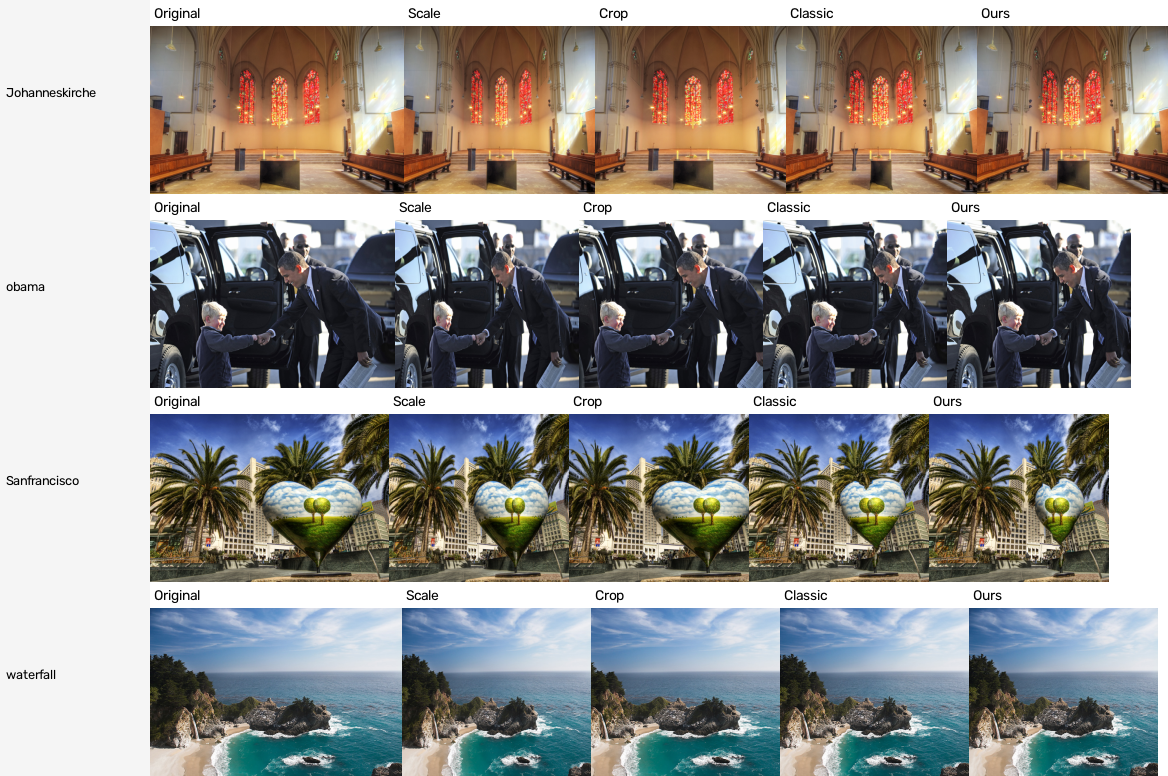
\includegraphics[width=\textwidth]{fig_compare_75_paper.png}
\caption{Width reduced to 75\%. Columns are the original, uniform scale, center crop, classic seams, and the full model.}
\label{fig:compare75}
\end{figure*}

\begin{figure*}[t]
\centering
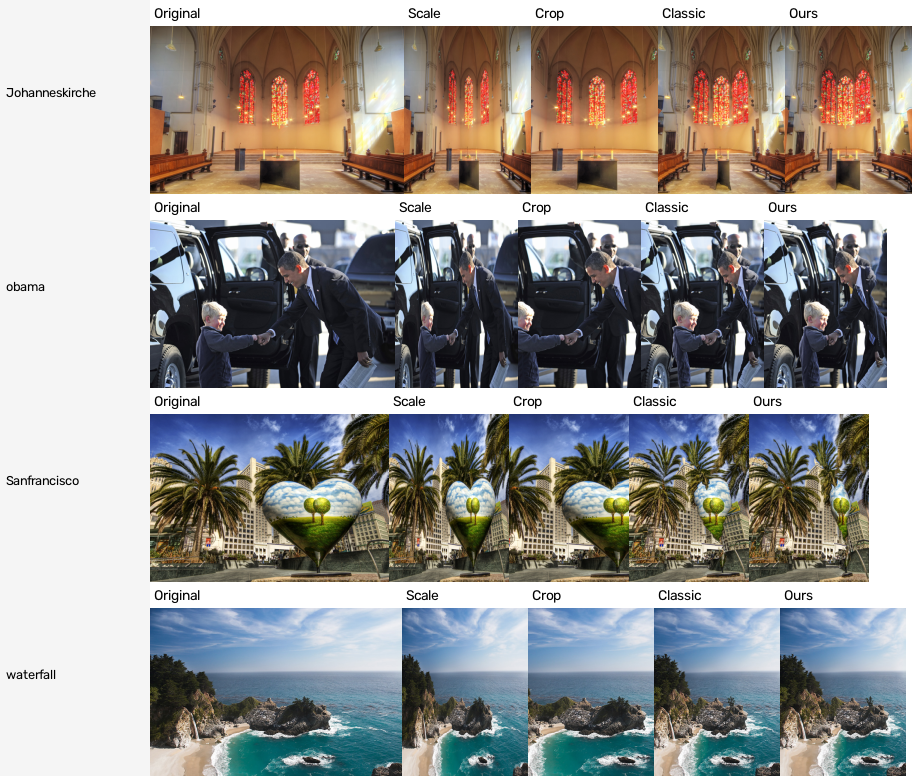
\includegraphics[width=\textwidth]{fig_compare_50_paper.png}
\caption{Width reduced to 50\% on the same four images. Any impression that one seam method bends a window or an outline less than the other is qualitative. The measured claims are the scores in Tables~\ref{tab:width75}--\ref{tab:perimage}.}
\label{fig:compare50}
\end{figure*}

\begin{figure}[t]
\centering
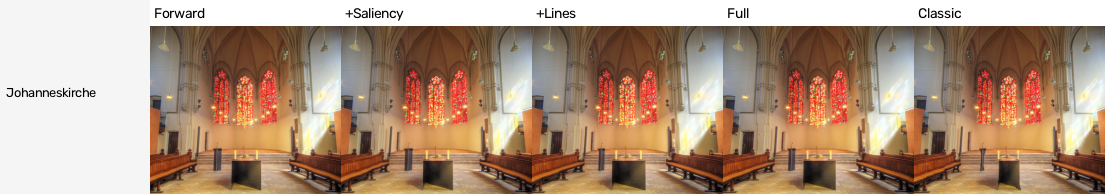
\includegraphics[width=\linewidth]{fig_ablation.png}
\caption{Ablation on Johanneskirche at 75\% width. Forward energy alone, forward energy plus saliency, forward energy plus lines, the full model, and classic backward energy.}
\label{fig:ablation}
\end{figure}

\begin{figure}[t]
\centering
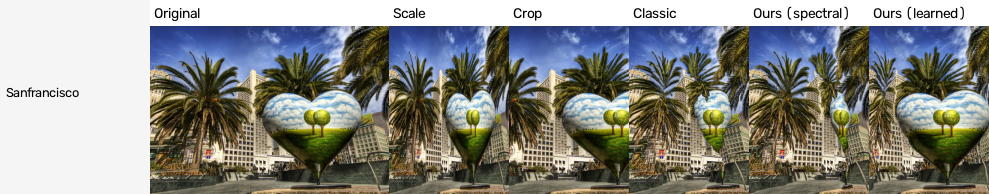
\includegraphics[width=\linewidth]{fig_failure.png}
\caption{Failure case. \texttt{Sanfrancisco} at 50\% width. The crop cuts the heart, scaling squeezes it, and both seam methods pinch the curved outline. The Hough map does not protect that curve.}
\label{fig:failure}
\end{figure}

\begin{figure*}[t]
\centering
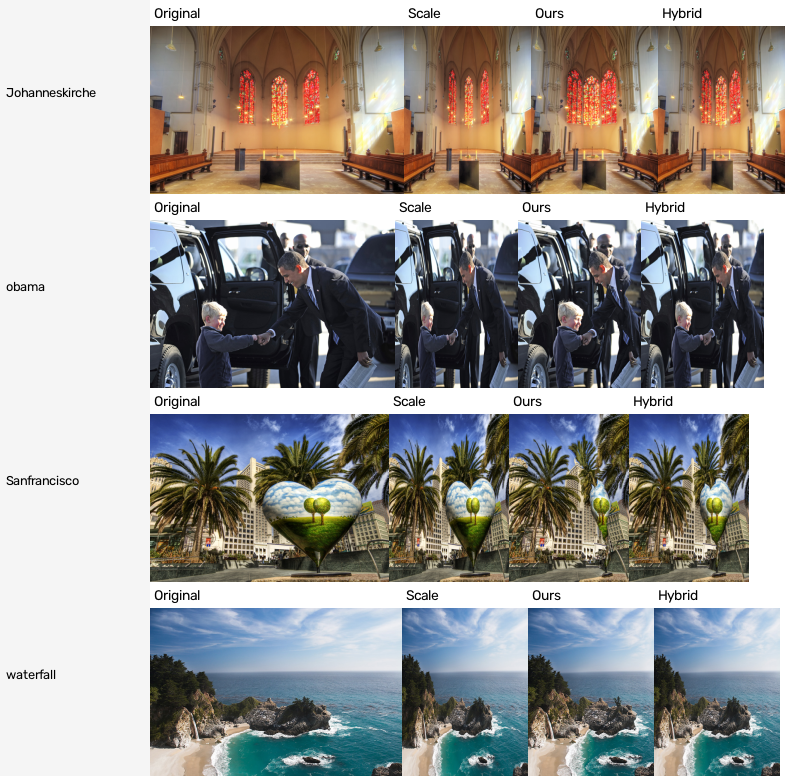
\includegraphics[width=\textwidth]{fig_hybrid_50.png}
\caption{Width reduced to 50\%. Columns are the original, uniform scale, the full model carved all the way, and hybrid (seams until 75\% of the original width, then scale). Hybrid avoids only the damage that the extra seams would add past 75\%.}
\label{fig:hybrid}
\end{figure*}

\begin{figure}[t]
\centering
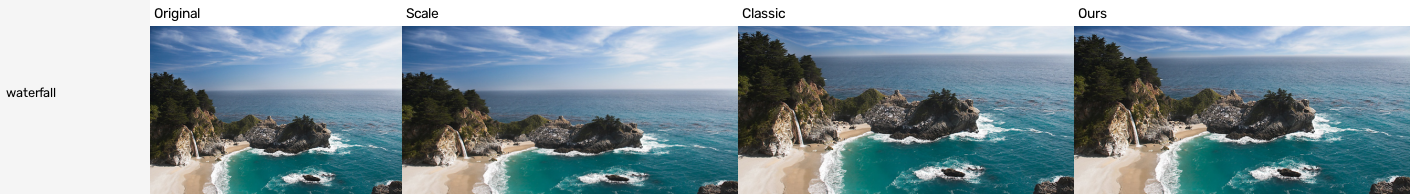
\includegraphics[width=\linewidth]{fig_height.png}
\caption{Height reduced to 75\% on \texttt{waterfall}. Horizontal seams use the line map weighted by $|\cos\theta|$.}
\label{fig:height}
\end{figure}

\begin{figure}[t]
\centering
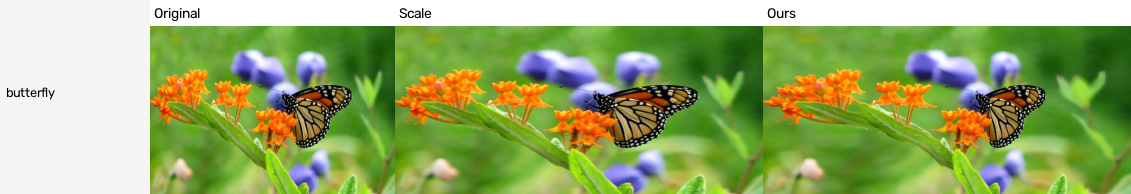
\includegraphics[width=\linewidth]{fig_enlarge.png}
\caption{Width enlarged to 150\% on \texttt{butterfly}. Seams are recorded by removal and inserted as averaged duplicates.}
\label{fig:enlarge}
\end{figure}

The full eight-image contact sheets are Figures~\ref{fig:all75} and~\ref{fig:all50} in the appendix.
Across the 75\% and 50\% trials, every output size matched the requested size.

\subsection{What the demo shows}
The Gradio application loads an image, caps the long side at 640 pixels, and takes the target size as a percentage of that working image.
The user picks scale, crop, classic, the full model, or the hybrid schedule, and moves $w_s$ and $w_l$.
Optional panels show the saliency map, the vertical-seam line map, and the next vertical seam.
Three examples are wired to the roles above: Johanneskirche for lines, obama for a person, and Sanfrancisco for the busy failure.
A useful order in a presentation is to raise $w_l$ on the church, compare classic and the full model on the portrait, and then set the street scene to 50\% width and say plainly what every method loses.

\subsection{Learned saliency comparison}
The learned map is U$^2$-Net-small, loaded through \texttt{rembg} as the \texttt{u2netp} checkpoint \cite{qin2020u2net}.
It is pretrained. We did not train it.
Its output is near-binary, so in the seam cost it acts like a mask.
The spectral default remains $w_s = 0.5$ and $w_l = 0.8$.
For the learned source, $w_l = 0.8$ and $w_s = 0.25$.
That $0.25$ was the smallest of the five weights $\{0.25, 0.5, 1, 2, 4\}$ tested on Johanneskirche and \texttt{obama} only.
Every tested weight put the learned-mass fraction below half the forward-only value on both images, and the fraction of seam pixels above $0.5$ on the learned map was 0 at every tested weight.
\texttt{obama} is one of the two tuning images, and its learned map marks the car door rather than the people, so this weight is not evidence that people are protected.
Ours learned always includes the line weight.
It is compared with forward plus lines and with ours spectral, which also use $w_l = 0.8$.
It is not compared with forward-only, because that comparison confounds the line weight.
Ours learned uses $w_s = 0.25$ and ours spectral uses $w_s = 0.5$, so the comparison is also not a pure swap of the map.
Each source is expected to score better under its own map.
On the 30-image sample, ours spectral scores 0.093 (0.031) under the spectral map and 0.179 (0.138) under the learned map.
Ours learned scores 0.144 (0.052) under the spectral map and 0.030 (0.053) under the learned map.
Against ours spectral under the spectral map, ours learned is lower on 0 images, higher on 30, and tied on 0 ($p = 1.86 \times 10^{-9}$). This does not show that learned-chosen seams are better on this map. Against ours spectral under the learned map, ours learned is lower on 30 images, higher on 0, and tied on 0 ($p = 1.86 \times 10^{-9}$). The sign test favors ours learned on this map. Against forward + lines under the spectral map, ours learned is lower on 11 images, higher on 19, and tied on 0 ($p = 0.2005$). This does not show that learned-chosen seams are better on this map. Against forward + lines under the learned map, ours learned is lower on 30 images, higher on 0, and tied on 0 ($p = 1.86 \times 10^{-9}$). The sign test favors ours learned on this map.
Tables~\ref{tab:learned8} and~\ref{tab:learned30} are the 75\% width cross-evaluation.
Table~\ref{tab:learned850} is the same six methods on the original eight at 50\% width.
The earlier full sheets are Figures~\ref{fig:all75} and~\ref{fig:all50}.
The same eight images with ours spectral and ours learned are Figures~\ref{fig:learnedall75} and~\ref{fig:learnedall50}.
The 30-image sample is Figures~\ref{fig:n30a} and~\ref{fig:n30b}, in alphabetical order.
Those sheets are impressions, not measurements, and the images were not selected by outcome.
Figure~\ref{fig:learnedsf} is \texttt{Sanfrancisco} at 50\% width, and Figure~\ref{fig:learnedset} is \texttt{brick\_house}, \texttt{child}, and \texttt{obama} at the same width.
Both are impressions, not measurements.
Blob is the fraction of seam pixels whose learned-map value is above 0.5.
\begin{table*}[t]
\centering
\caption{Original eight at 75\% width. Spectral and Learned are fractions of that map deleted. Hough and LSD are crossings per 100 seam pixels. Blob is the fraction of seam pixels with learned value above 0.5. Ours learned uses $w_s = 0.25$ and $w_l = 0.8$. Ours spectral uses $w_s = 0.5$ and $w_l = 0.8$.}
\label{tab:learned8}
\scriptsize
\begin{tabular}{lccccc}
\toprule
Method & Spectral & Learned & Hough & LSD & Blob \\
\midrule
Classic & 0.089 (0.045) & 0.192 (0.155) & 1.30 (1.25) & 1.45 (0.73) & 0.120 (0.135) \\
Forward only & 0.089 (0.039) & 0.196 (0.172) & 1.14 (1.18) & 1.28 (0.55) & 0.141 (0.182) \\
Forward + lines & 0.089 (0.040) & 0.212 (0.212) & 0.31 (0.22) & 1.27 (0.53) & 0.157 (0.207) \\
Ours spectral & 0.068 (0.036) & 0.210 (0.225) & 0.37 (0.31) & 1.26 (0.54) & 0.159 (0.219) \\
Learned saliency only & 0.114 (0.081) & 0.005 (0.008) & 2.16 (3.05) & 1.02 (0.65) & 0.002 (0.005) \\
Ours learned & 0.118 (0.086) & 0.005 (0.009) & 0.94 (1.46) & 0.98 (0.62) & 0.002 (0.005) \\
\bottomrule
\end{tabular}
\end{table*}
\begin{table*}[t]
\centering
\caption{Seeded 30-image sample at 75\% width, seed 604. Johanneskirche and \texttt{obama} were not drawn. Columns match Table~\ref{tab:learned8}. Ours learned is not claimed to be better unless the sign tests say so.}
\label{tab:learned30}
\scriptsize
\begin{tabular}{lccccc}
\toprule
Method & Spectral & Learned & Hough & LSD & Blob \\
\midrule
Classic & 0.118 (0.037) & 0.167 (0.108) & 1.70 (1.45) & 1.08 (0.93) & 0.156 (0.191) \\
Forward only & 0.121 (0.035) & 0.184 (0.119) & 2.07 (1.75) & 1.35 (1.37) & 0.174 (0.205) \\
Forward + lines & 0.122 (0.036) & 0.183 (0.129) & 0.94 (0.75) & 1.16 (0.94) & 0.171 (0.211) \\
Ours spectral & 0.093 (0.031) & 0.179 (0.138) & 1.03 (0.86) & 1.26 (1.10) & 0.172 (0.212) \\
Learned saliency only & 0.145 (0.054) & 0.029 (0.052) & 2.27 (2.03) & 1.29 (1.37) & 0.052 (0.132) \\
Ours learned & 0.144 (0.052) & 0.030 (0.053) & 1.17 (0.98) & 1.10 (0.96) & 0.053 (0.137) \\
\bottomrule
\end{tabular}
\end{table*}
\begin{table*}[t]
\centering
\caption{Original eight at 50\% width. Same columns and weights as Table~\ref{tab:learned8}.}
\label{tab:learned850}
\scriptsize
\begin{tabular}{lccccc}
\toprule
Method & Spectral & Learned & Hough & LSD & Blob \\
\midrule
Classic & 0.222 (0.097) & 0.377 (0.225) & 1.61 (1.34) & 1.47 (0.60) & 0.127 (0.116) \\
Forward only & 0.231 (0.087) & 0.395 (0.240) & 1.56 (1.28) & 1.33 (0.53) & 0.142 (0.138) \\
Forward + lines & 0.224 (0.097) & 0.403 (0.301) & 0.63 (0.48) & 1.28 (0.50) & 0.147 (0.156) \\
Ours spectral & 0.186 (0.090) & 0.400 (0.314) & 0.69 (0.56) & 1.29 (0.52) & 0.147 (0.164) \\
Learned saliency only & 0.288 (0.183) & 0.037 (0.046) & 2.50 (3.01) & 1.25 (0.64) & 0.011 (0.018) \\
Ours learned & 0.285 (0.179) & 0.048 (0.044) & 1.58 (1.98) & 1.21 (0.60) & 0.015 (0.018) \\
\bottomrule
\end{tabular}
\end{table*}
\begin{figure*}[t]
\centering
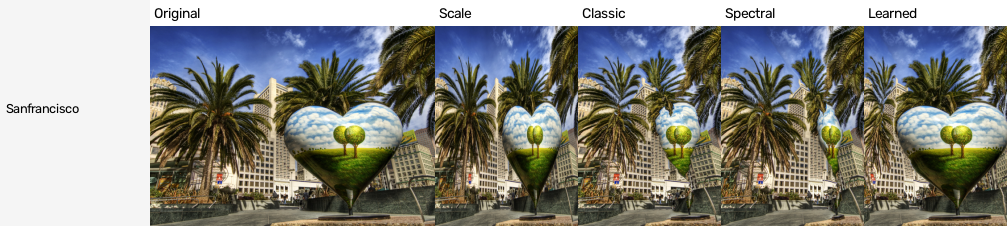
\includegraphics[width=\textwidth]{fig_learned_sf50.png}
\caption{\texttt{Sanfrancisco} at 50\% width. Columns are the original, uniform scale, classic seams, ours spectral, and ours learned. Any impression that the heart is preserved is not a measurement.}
\label{fig:learnedsf}
\end{figure*}
\begin{figure*}[t]
\centering
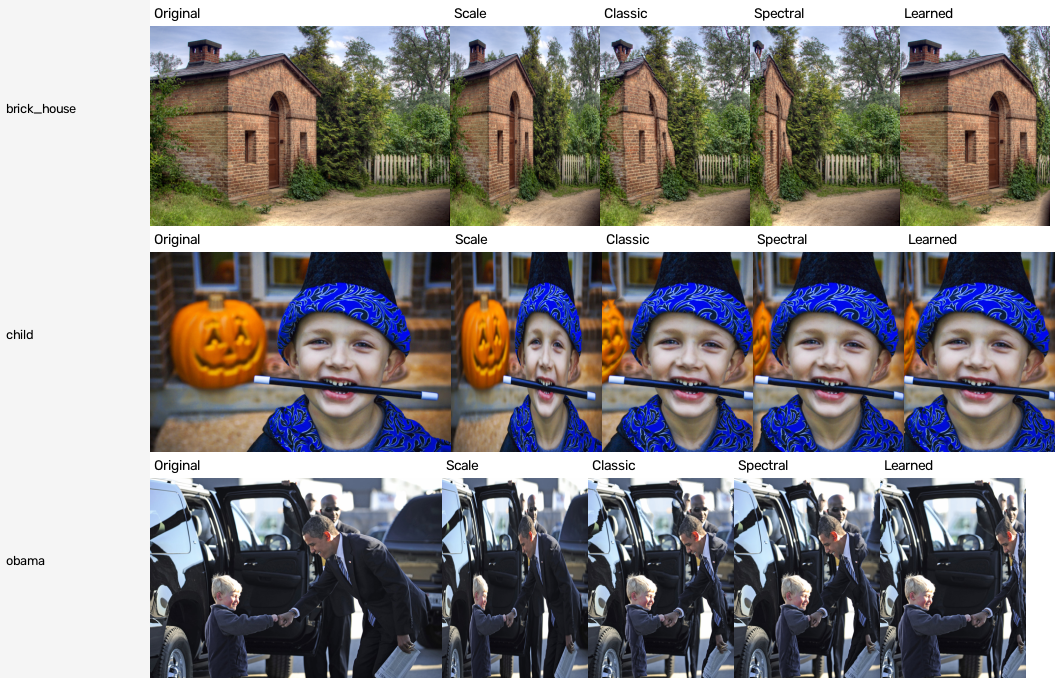
\includegraphics[width=\textwidth]{fig_learned_50_set.png}
\caption{\texttt{brick\_house}, \texttt{child}, and \texttt{obama} at 50\% width, with the same columns as Figure~\ref{fig:learnedsf}. These sheets are impressions, not measurements. The \texttt{obama} learned map marks the car door rather than the people.}
\label{fig:learnedset}
\end{figure*}

\subsection{Limitations}
The saliency score and the Hough line score reuse the maps inside the cost.
A lower score shows that the corresponding weight changed the seam.
It does not show that the deleted pixels were less important to a viewer, and pushing seams off those maps can tear texture that neither map marks.
A pretrained saliency model is reported as an optional comparison. No summed forward-energy of the chosen seams is reported.
One independent check is reported: the same seams are counted on an LSD line map that is not in the cost.
On the original eight that score moves much less than the Hough score.
On the seeded 30 it does not favor the full model over classic seams, and the line weight does not win a sign test against forward energy.
Spectral residual saliency responds strongly to edges and is not a subject detector. The optional learned comparison is a pretrained salient-object model \cite{qin2020u2net}.
The line map only contains segments the Hough transform returns, so short and curved structures, including the heart sculpture, are unprotected except where the residual happens to be high.
A strong-edge penalty does not fix that curve: the seam pays it at the crossing and then follows the cheap interior.
The hybrid schedule stops further seam cuts after 75\%, which is not the same as protecting the object during the first 25\%.
The spectral weights were chosen on two of the eight test images, and they were not swept.
Those two were not in the 30-image draw.
The line-score standard deviation is about as large as the mean on both the eight and the 30.
Thirty images is still not the full RetargetMe set.
The comparison does not include the published RetargetMe operators, such as multi-operator search, shift-map, or warping.
Hybrid is a fixed seam-then-scale schedule, not that search.
The height cut and the enlargement are single images.
Runtimes are one measurement each.
There is no user study.

\section{Conclusion}
The operator is forward-energy seam carving plus a spectral-residual term and an orientation-weighted line term.
On eight RetargetMe images, turning the terms off one at a time moves two different scores, and both scores are built from the maps in the cost.
The saliency weight lowers deleted residual mass from 0.089 to 0.068.
On the seeded 30 images the full model is lower than classic on that fraction for every image, 0.093 (0.031) against 0.118 (0.037).
The line weight lowers Hough-map crossings from 1.14 to 0.31 per 100 seam pixels.
The full model keeps the saliency-score reduction and most, not all, of that Hough reduction: its Hough score is 0.37 rather than 0.31.
Leaving out the two images used to pick the weights does not remove that Hough and saliency separation on the other six.
That is evidence that those weights move the maps they were built from.
On the original eight, an LSD map that is not in the cost puts the full model only about 13\% below classic seams, and only on four of the eight images, and adding the line weight to forward energy does not lower that score.
On the seeded sample of 30 the LSD mean goes the other way, 1.26 against 1.08, and the sign tests do not show a benefit ($p = 0.46$ for the full model against classic, $p = 0.71$ for the line weight against forward energy).
The Hough score on those 30 images still falls, which is what a map inside the cost is expected to do.
It is not evidence that the results look better, that subjects are preserved, or that the method beats other published retargeting operators.
Scaling and cropping are the simple baselines.
A large reduction of a busy curved scene still damages the content.
Stopping the seams at 75\% and scaling the rest removes only the extra damage that comes from carving on to half width.
It does not put the curved sculpture back to the shape that uniform scaling keeps.
On the learned comparison, each source wins under its own map.
The one fair comparison, ours learned against forward plus lines under the spectral map, is not significant ($p = 0.20$).
By eye, the learned map kept the heart on \texttt{Sanfrancisco} and squeezed the man on \texttt{obama}.

{
\small
\bibliographystyle{ieeenat_fullname}
\bibliography{main}
}

\appendix
\onecolumn

\section{Individual contributions}
\subsection{230991}
I implemented the luminance, spectral-residual saliency, and orientation-aware line maps; the forward-energy and classic backward-energy dynamic programs, including seam removal and insertion; the scaling and center-crop baselines; the hybrid schedule that stops seams at 75\% of a side; the RetargetMe experiments and figures; the Gradio demo; and this write-up.

\section{Links}
The source images are the RetargetMe archive of Rubinstein et al.:
\url{http://people.csail.mit.edu/mrub/retargetme/}
and the file linked as ``source images only'' from
\url{http://people.csail.mit.edu/mrub/retargetme/download.html}.
The libraries are OpenCV (\url{https://github.com/opencv/opencv}),
NumPy (\url{https://github.com/numpy/numpy}),
and Gradio (\url{https://github.com/gradio-app/gradio}).
The complete source is printed in the next section and included with this submission.
No public repository link is attached.

\section{All eight images}
\begin{figure}[h]
\centering
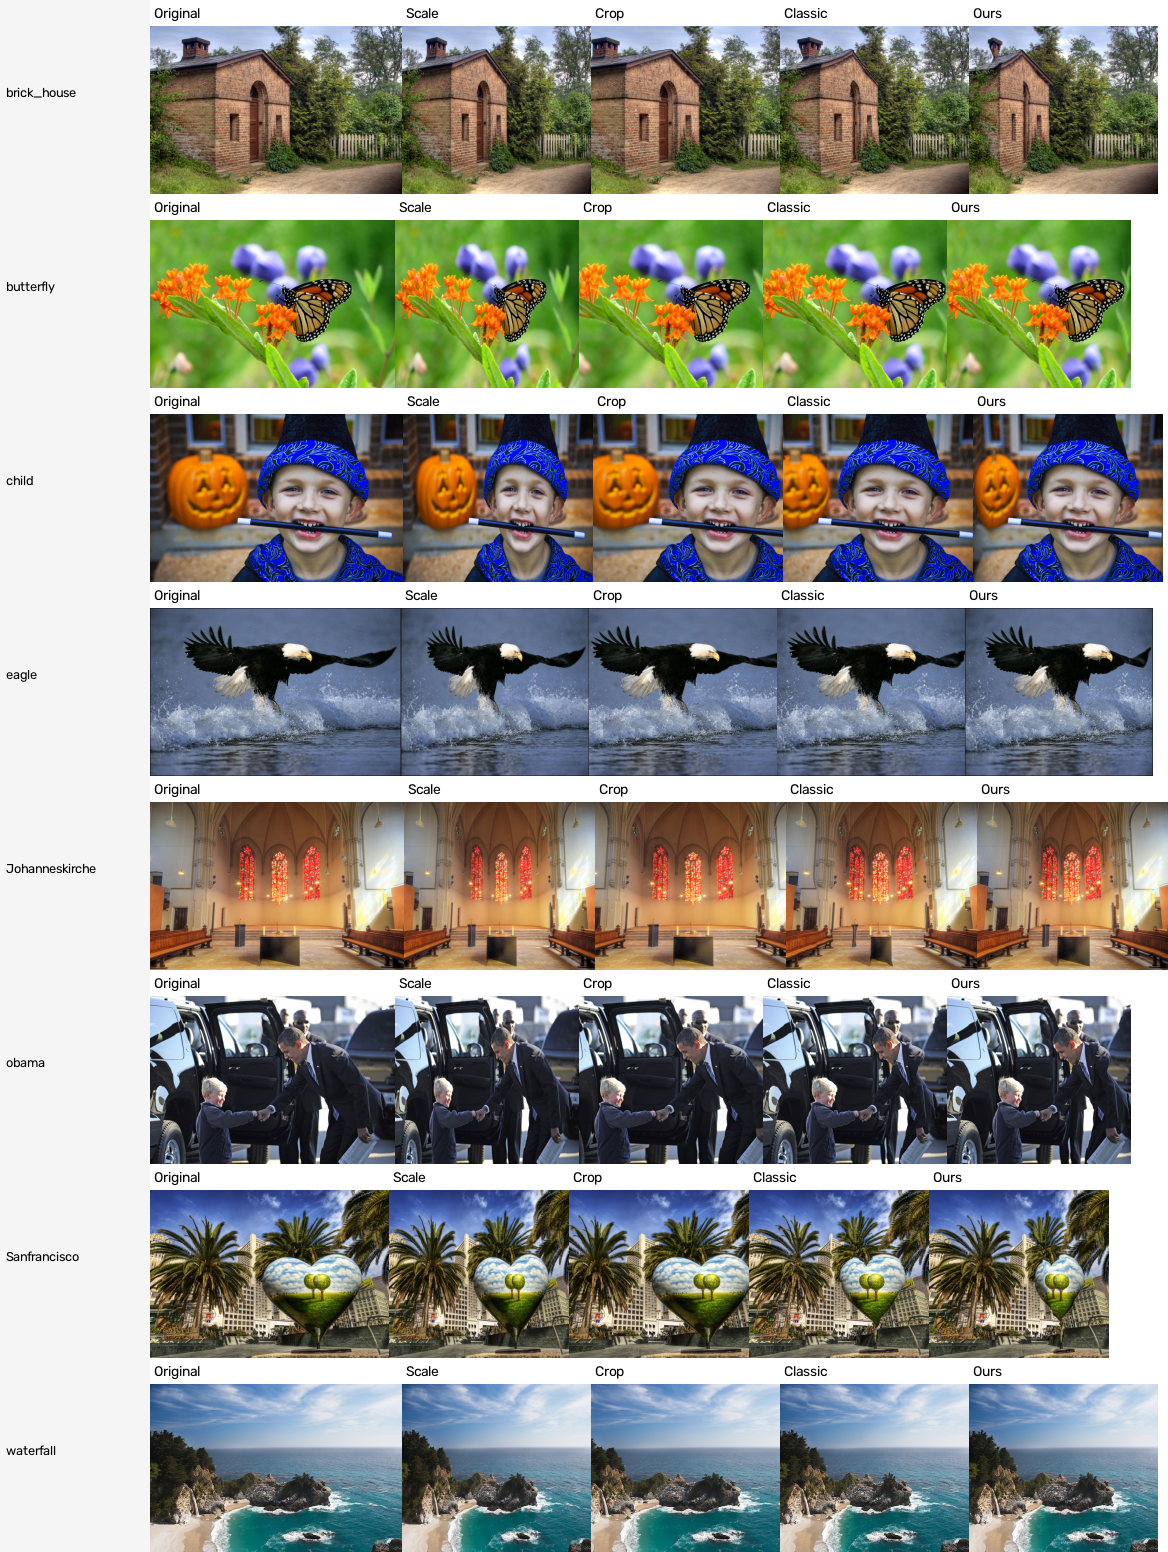
\includegraphics[width=\textwidth,height=0.78\textheight,keepaspectratio]{fig_compare_75.png}
\caption{All eight images at 75\% width. Columns are the original, scale, crop, classic seams, and the full model.}
\label{fig:all75}
\end{figure}

\begin{figure}[h]
\centering
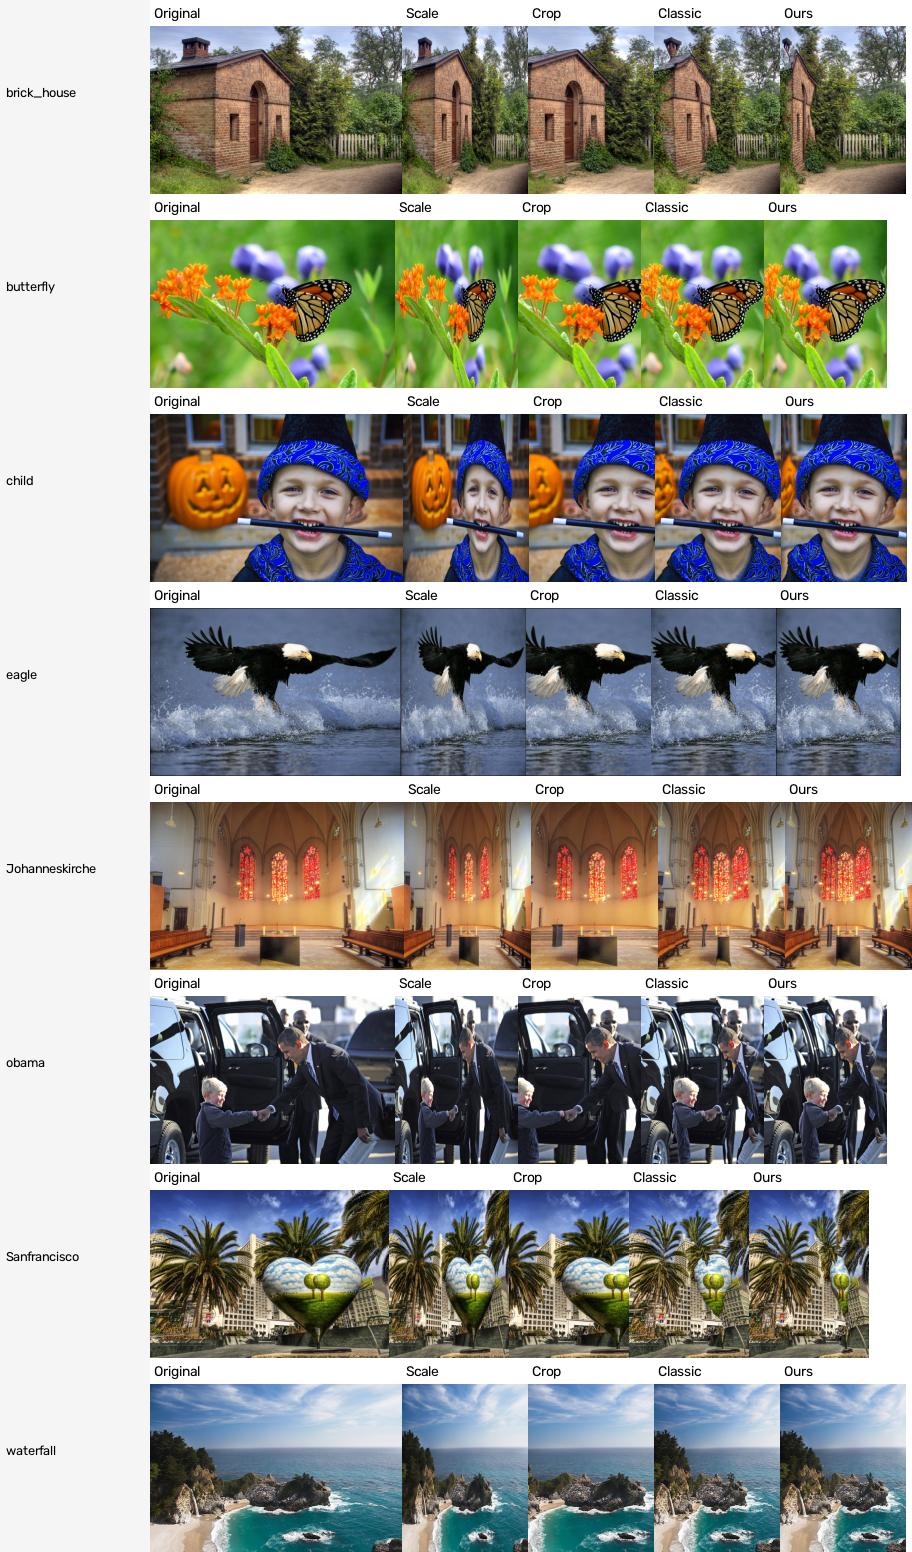
\includegraphics[width=\textwidth,height=0.78\textheight,keepaspectratio]{fig_compare_50.png}
\caption{All eight images at 50\% width.}
\label{fig:all50}
\end{figure}

\begin{figure}[h]
\centering
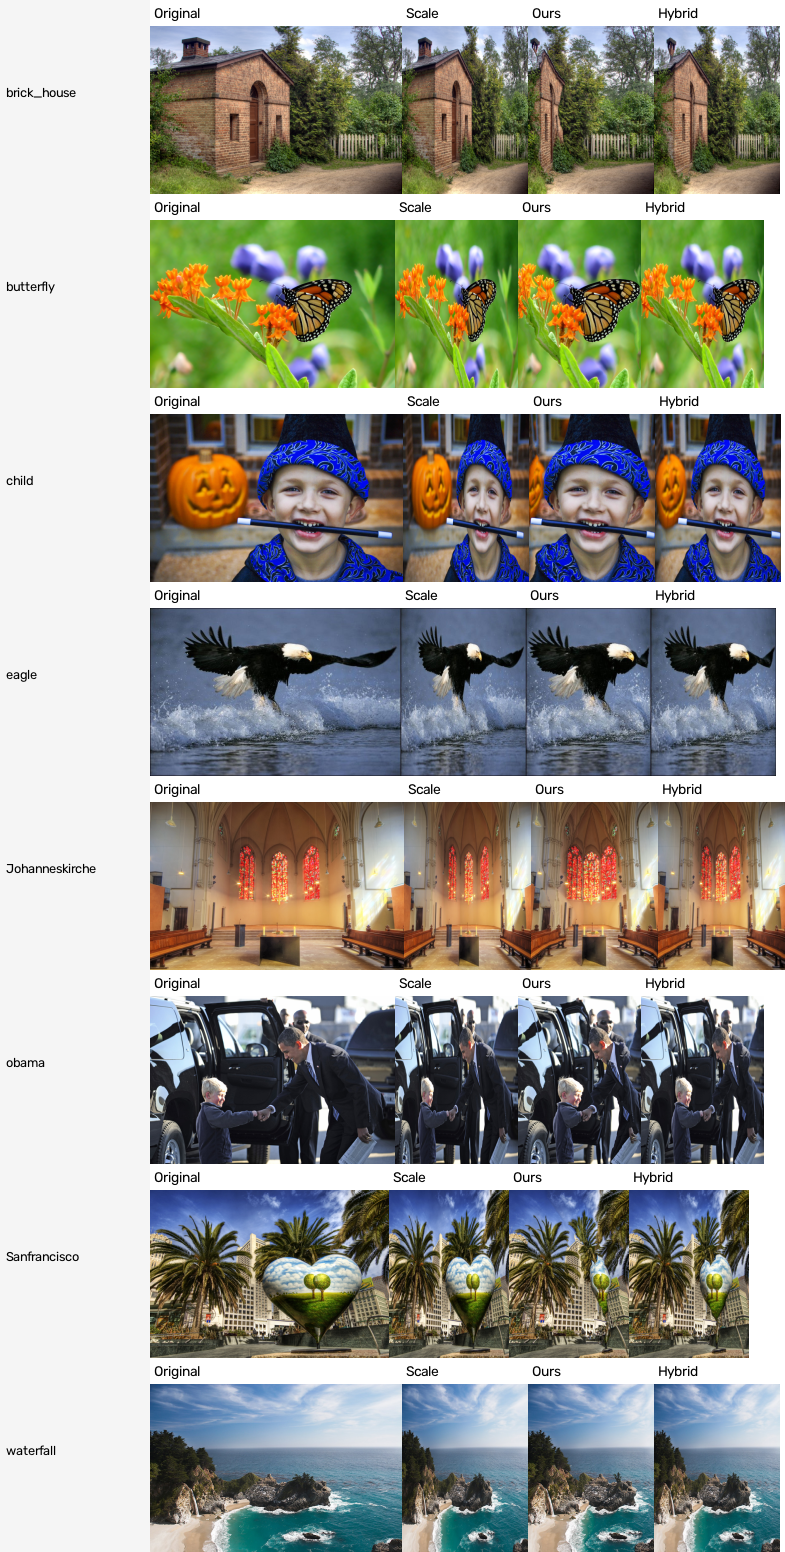
\includegraphics[width=\textwidth,height=0.78\textheight,keepaspectratio]{fig_hybrid_50_all.png}
\caption{All eight images at 50\% width. Columns are the original, uniform scale, the full model, and hybrid.}
\label{fig:hybridall}
\end{figure}

\section{Learned comparison sheets}
\begin{figure}[h]
\centering
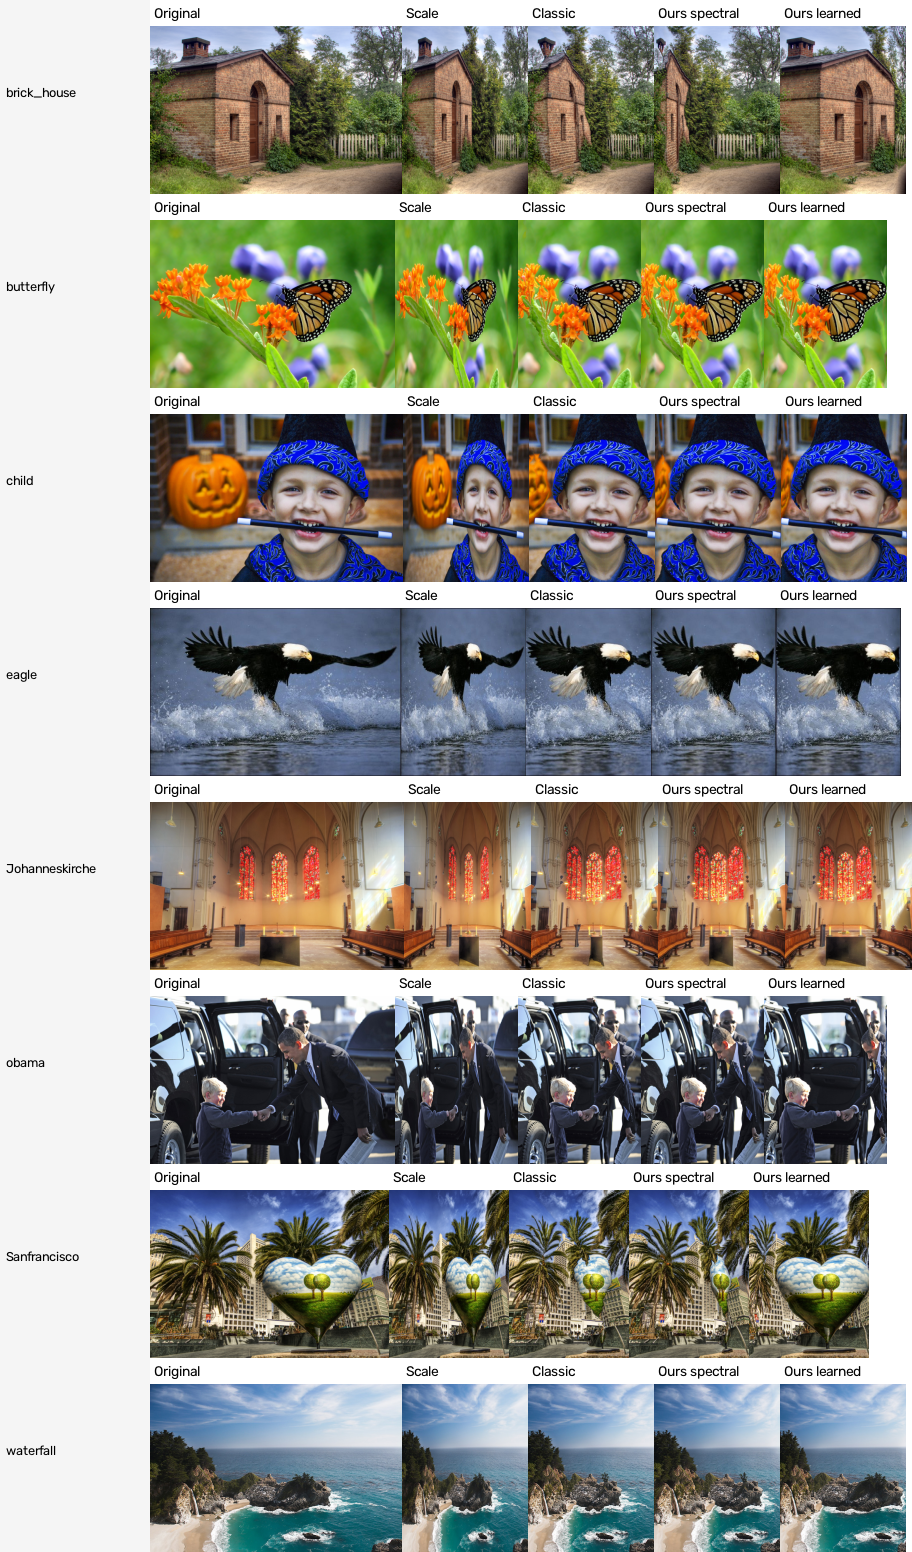
\includegraphics[width=\textwidth,height=0.78\textheight,keepaspectratio]{fig_learned_all50.png}
\caption{All eight original images at 50\% width, in the same order as Figures~\ref{fig:all75} and~\ref{fig:all50}. Columns are the original, uniform scale, classic seams, ours spectral, and ours learned. These are impressions, not measurements. The images were not selected by outcome.}
\label{fig:learnedall50}
\end{figure}

\begin{figure}[h]
\centering
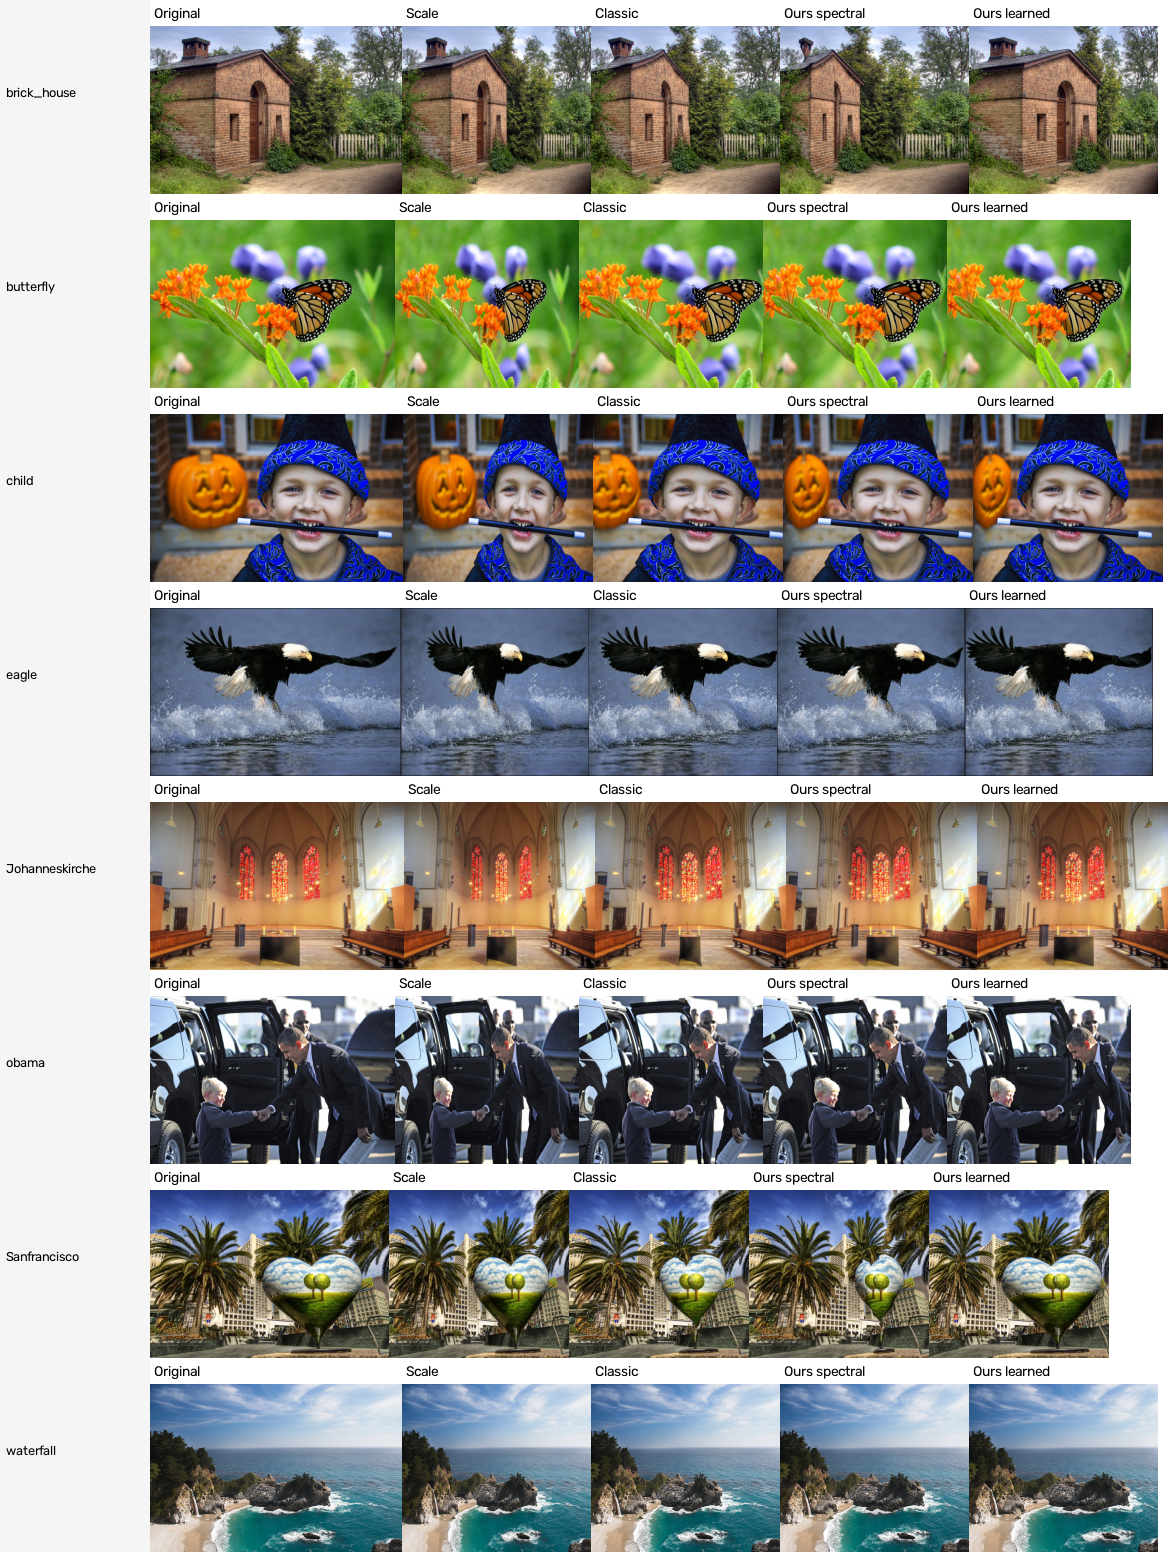
\includegraphics[width=\textwidth,height=0.78\textheight,keepaspectratio]{fig_learned_all75.png}
\caption{All eight original images at 75\% width. Columns match Figure~\ref{fig:learnedall50}. These are impressions, not measurements. The images were not selected by outcome.}
\label{fig:learnedall75}
\end{figure}

\begin{figure}[h]
\centering
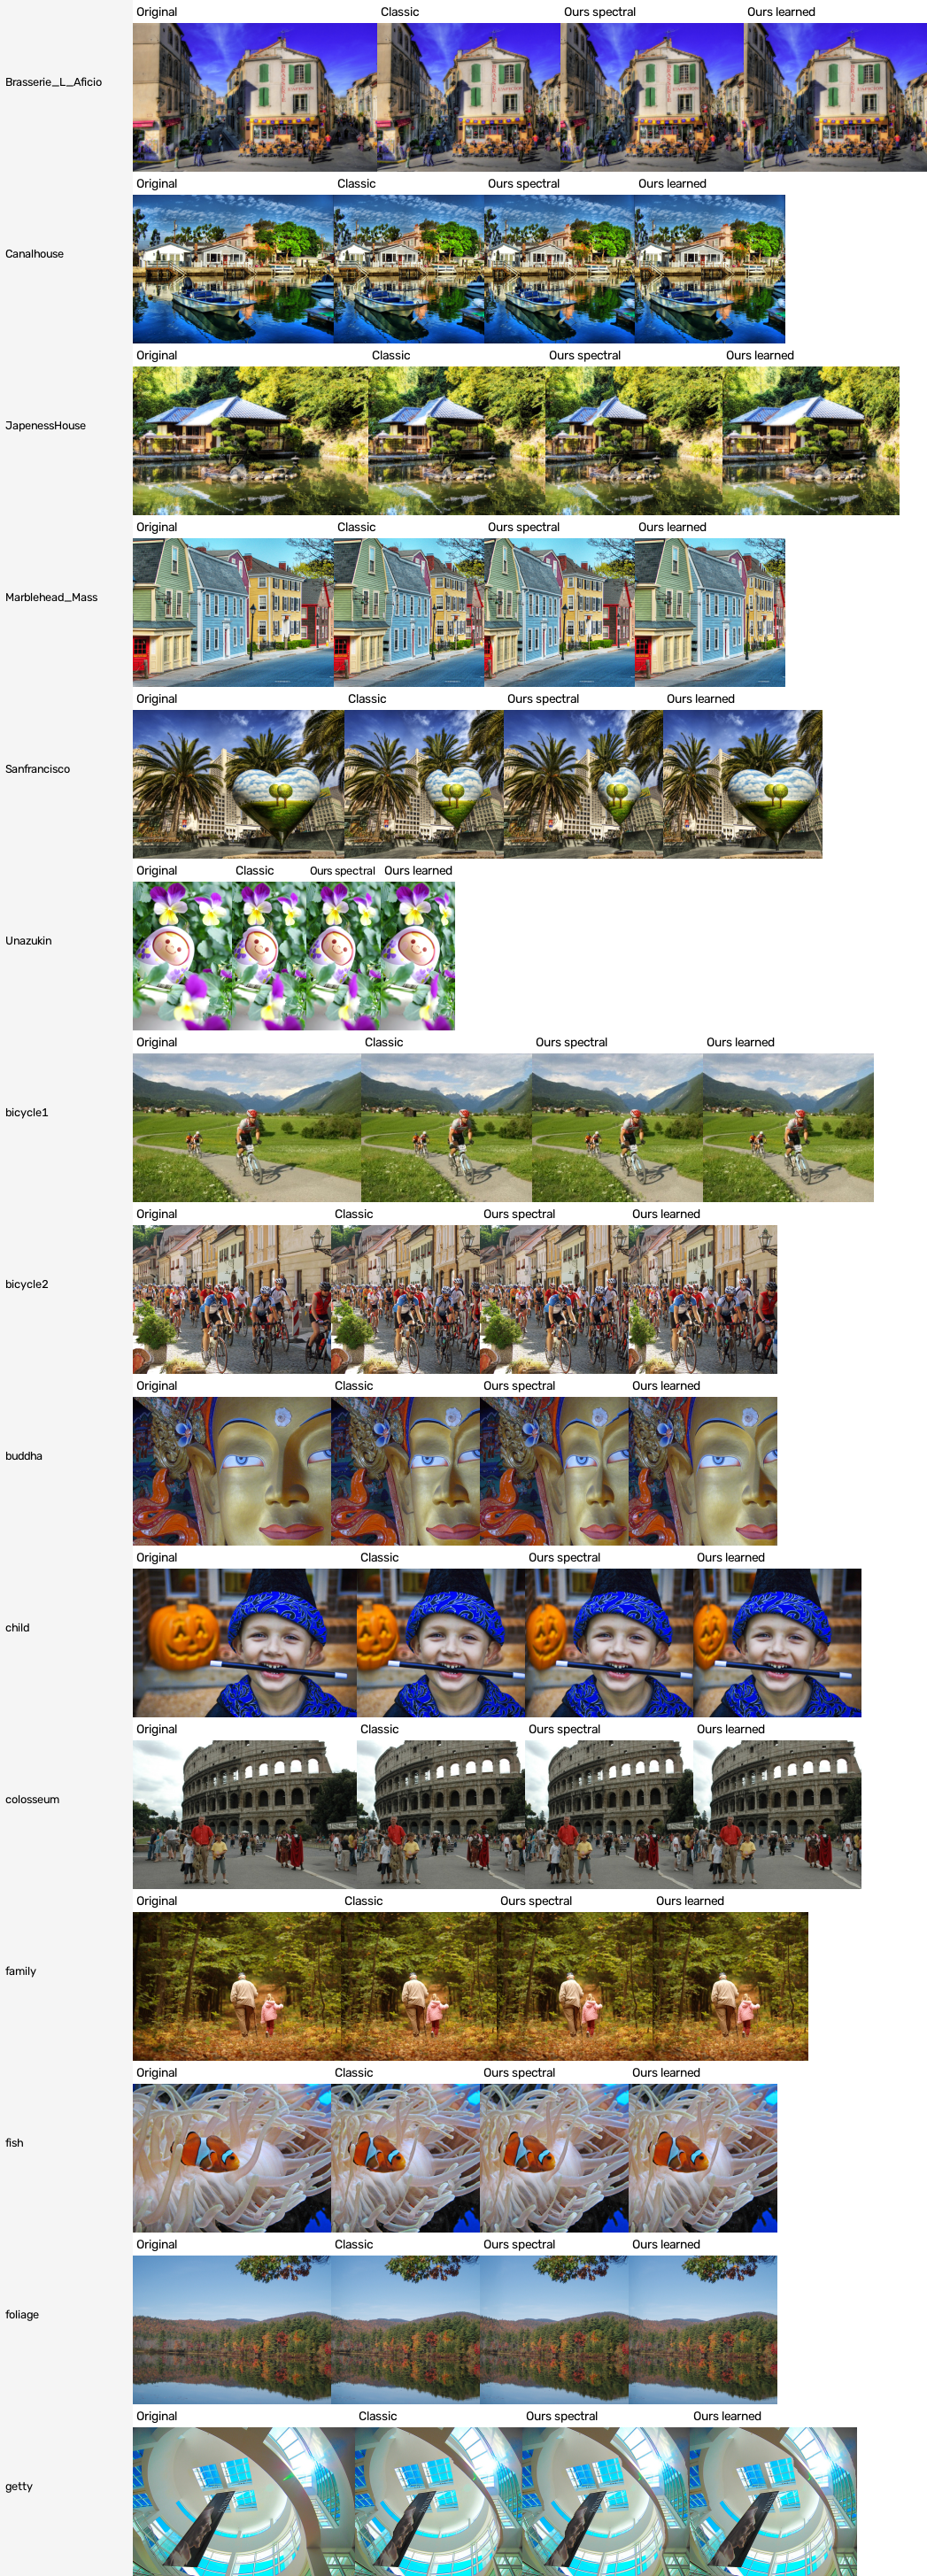
\includegraphics[width=\textwidth,height=0.78\textheight,keepaspectratio]{fig_n30_overview_a.png}
\caption{First 15 images of the seed-604 sample at 75\% width, alphabetical order. Columns are the original, classic seams, ours spectral, and ours learned. These are impressions, not measurements. The images were not selected by outcome.}
\label{fig:n30a}
\end{figure}

\begin{figure}[h]
\centering
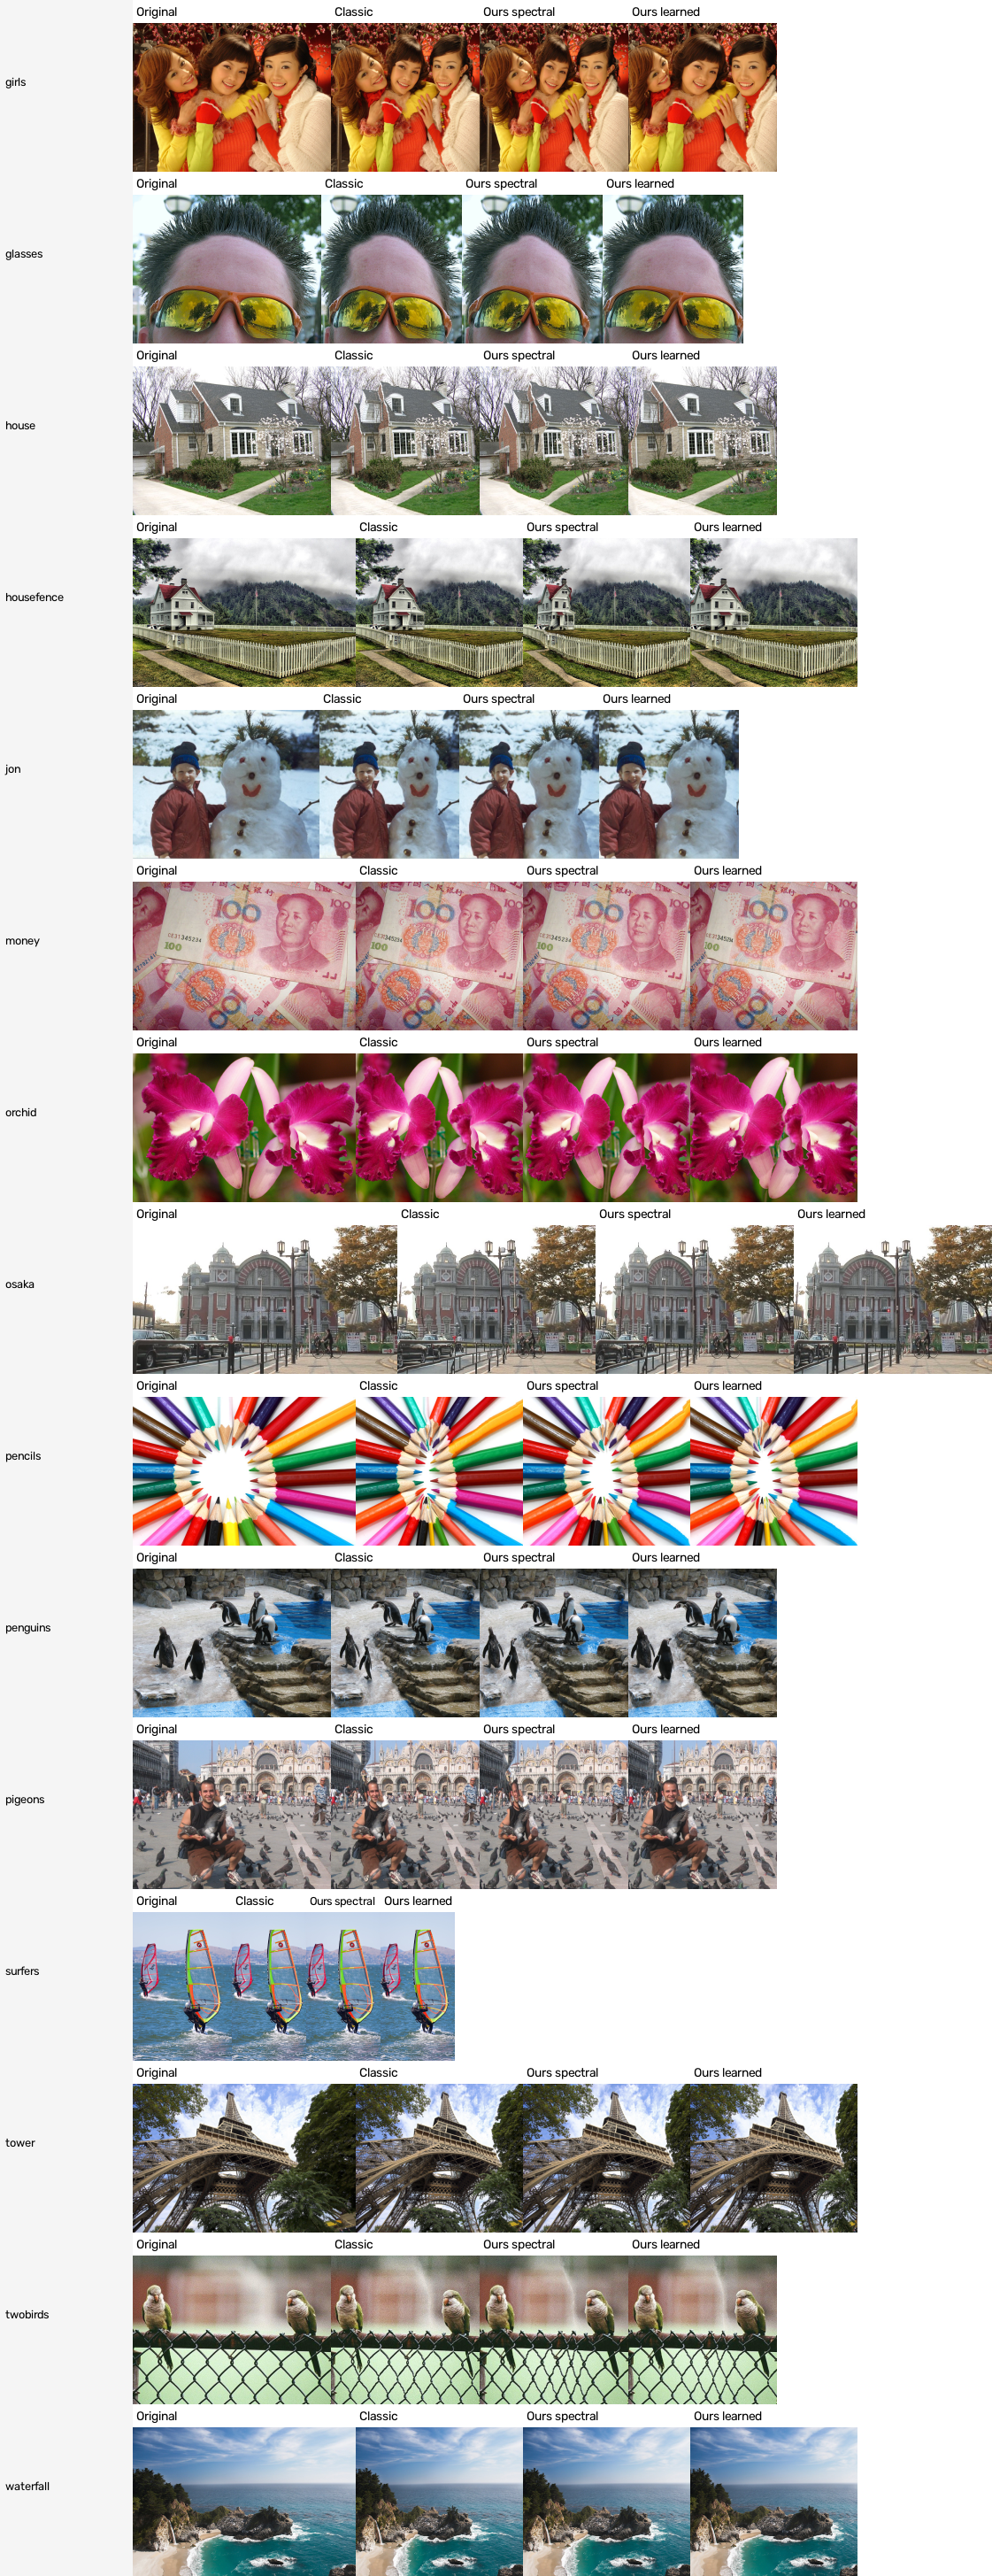
\includegraphics[width=\textwidth,height=0.78\textheight,keepaspectratio]{fig_n30_overview_b.png}
\caption{Remaining 15 images of the seed-604 sample at 75\% width, continuing the alphabetical order of Figure~\ref{fig:n30a}. Columns match that figure. These are impressions, not measurements. The images were not selected by outcome.}
\label{fig:n30b}
\end{figure}

\section{Source code}
The listings below are the program submitted with this report.
They match the source included with this submission.

\begingroup
\catcode`\_=12
\lstinputlisting[caption={src/__init__.py}]{../src/__init__.py}
\endgroup
\lstinputlisting[caption={src/energy.py}]{../src/energy.py}
\lstinputlisting[caption={src/seam.py}]{../src/seam.py}
\lstinputlisting[caption={src/baselines.py}]{../src/baselines.py}
\lstinputlisting[caption={src/retarget.py}]{../src/retarget.py}
\lstinputlisting[caption={src/metrics.py}]{../src/metrics.py}
\lstinputlisting[caption={src/display.py}]{../src/display.py}
\lstinputlisting[caption={app.py}]{../app.py}
\begingroup
\catcode`\_=12
\lstinputlisting[caption={experiments/download_retargetme.py}]{../experiments/download_retargetme.py}
\lstinputlisting[caption={experiments/run_experiments.py}]{../experiments/run_experiments.py}
\lstinputlisting[caption={experiments/run_hybrid.py}]{../experiments/run_hybrid.py}
\lstinputlisting[caption={experiments/report_numbers.py}]{../experiments/report_numbers.py}
\lstinputlisting[caption={experiments/score_lsd.py}]{../experiments/score_lsd.py}
\lstinputlisting[caption={experiments/run_n30.py}]{../experiments/run_n30.py}
\endgroup

\end{document}
